\section{Andre datastrukturer}
\subsection{Heap (prioritetskø)}\label{heap}
En heap (også kalt prioritetskø) er en type binært tre med noen spesielle struktur- og ordningskrav. Vi har to typer heap: min- og maksheap. Vi vil beskrive minheap i dette kapitlet, men maksheap fremgår helt analogt.

\begin{definisjon} En minheap er et binært tre der følgende krav er oppfylt:  \label{def:heap}
\begin{enumerate}
\item Treet er komplett (høyden til treet er $ \lceil\log_2 n\rceil $)
\item En node har alltid (sorterings)verdi mindre enn, eller lik sine barn. 
\end{enumerate}
\end{definisjon}

En maksheap defineres nesten likt, eneste forskjell er at pt. 2 i definisjonen blir ``En node alltid er større enn, eller lik sine barn.''

Hver node i en heap inneholder to ting: et element, og en verdi vi sorterer etter. I motsetning til i et binært søketre der vi sorterer på elementet selv, vil vi med en heap tilordne en sorteringsverdi til hvert element som ikke trenger å ha noe med elementet å gjøre. 

~\\
\begin{figure}[H]
\centering
\caption{En (min)heap. For oversiktens skyld er kun sorteringsverdiene tatt med.}
\label{fig:heap}
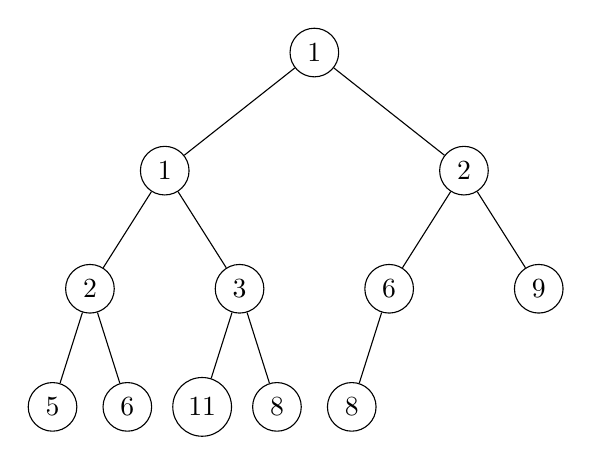
\begin{tikzpicture}[level distance=1.5cm,
  level 1/.style={sibling distance=3.8cm},
  level 2/.style={sibling distance=1.9cm},
  level 3/.style={sibling distance=0.95cm},
every node/.style = {shape=circle, draw, align=center}]

\node{1}
	child {node {1}
		child {node {2}
			child {node {5}}
			child {node {6}}
		}
		child {node {3}
			child {node {11}}
			child {node {8}}
		}
	}
	child {node {2}
		child {node {6}
			child {node {8}}
			child [missing] {}
		}
		child {node {9}}
	};
\end{tikzpicture}
\end{figure}

\paragraph{Innsetting}~\\
Når vi skal sette inn et element i en heap setter vi den på første ledige plassen. Deretter sammenligner vi nodens verdi med forelderens verdi. Hvis forelderen har større verdi enn noden vi setter inn bytter vi plass\footnote{Foreleser og lærebok kaller denne prosessen \say{percolate up}}. Så sammenligner vi med den nye forelderen, bytter plass om nødvendig, og fortsetter slik til enten forelderen er mindre enn noden, eller at noden er rot. 

\paragraph{Fjerning (deleteMin)}~\\
I en heap er vi egentlig bare interessert i å ta ut det minste elementet fra en heap (hvorfor blir diskutert i avsnittet om anvendelser). På grunn av krav 2 i definisjonen vet vi at rota er det minste elementet i heapen. Derfor fjerner vi rota. For å skaffe en ny rot tar vi det siste elementet i heapen og setter som rot. Deretter sammenligner vi verdien av den nye rota med verdien av barna. Hvis et (eller begge) av barna har mindre verdi enn den nye rota bytter rota plass med \textbf{det minste} barnet\footnote{\say{percolate down}}. Vi fortsetter slik til ordningskravet er oppfylt (noden har mindre verdi enn barna). 

\paragraph{Implementasjon}~\\
Vi kan implementere en heap som et tre (dvs, lage nodeobjekter med pekere til barn etc), men som oftest implementerer vi en heap ved hjelp av en array. Vi lar rota være på index 1. På grunn av kompletthetskravet kan vi legge nodene radvis bak rota. Vi finner da barna til en node på index $ i $ ved å til index $ 2i $ (venstre barn) og $ 2i+1 $ (høyre barn), og forelder ved å gå til index $ \lfloor i/2 \rfloor $. Når vi implementerer en heap som en array kan vi risikere å gå tom for plass i arrayen. Da må vi lage en ny array, og flytte over alle elementene til den nye arrayen. Vanligvis legger vi til en og en rad i slengen (eventuelt to og to, tre og tre, etc..). Å gjøre dette tar åpenbart $ O(n) $ tid, men vi må gjøre det sjeldnere og sjeldnere jo større heapen blir. 

\begin{figure}[H]
\centering
\caption{Heapen i fig \ref{fig:heap} representert som array}
\begin{tabular}{r||c|c|c|c|c|c|c|c|c|c|c|c|c|c|c|c}
	~~index &  0   & 1 & 2 & 3 & 4 & 5 & 6 & 7 & 8 & 9 & 10 & 11 & 12 &  13  &  14  &  15  \\ \hline
	~~verdi & null & 1 & 1 & 2 & 2 & 3 & 6 & 9 & 5 & 6 & 11 & 8  & 8  & null & null & null 
\end{tabular}
\end{figure}

I Java har vi en ferdig heap: \verb|java.util.PriorityQueue<E>|. Java krever at \verb|E| er sammenlignbar med seg selv (\verb|E| implementerer \verb|comparable<E>|) og vil bruke den sammenligningen som grunnlag for sortering. Javas heap er implementert som array. 

\paragraph{Tidsanalyse}~\\
Vi ser på kjøretiden til de to omtalte operajonene:
\begin{teorem} Kjøretid for heapoperasjoner \label{teo:heapop}
\begin{enumerate}[i]
\item Innsetting i en heap tar $ O(\log_2 n) $ tid
\item Fjerne minste element tar $ O(\log_2 n) $ tid
\end{enumerate}
\end{teorem}
Beviset følger av strukturkravet i definisjon \ref{def:heap}:
\begin{bevis} Teorem \ref{teo:heapop}, del i:

Når vi setter inn et element i en heap må vi først sette elementet på slutten av heapen. Siden vi vet hvor siste element er vil dette ta $ O(1) $ tid. Deretter må vi justere plassen til elementet ved å la elementet sive oppover. Siden treet er komplett vil høyden på treet være $ \lceil\log_2 n\rceil $, og vi kan maksimalt foreta $ \lceil\log_2 n\rceil - 1 $ byttinger. Total tid blir derfor være $ O(\log_2 n) $
\end{bevis}
Argumentet for teo. \ref{teo:heapop}, del ii er helt analogt. 


\paragraph{Anvendelser}~\\
I dette kurset ser vi på to anvendelser av en heap: Prioritetskø og sortering. Når vi bruker en (min)heap som en prioritetskø lar vi viktige jobber ha lav verdi, og mindre viktige jobber ha høy verdi. Når vi setter jobbene våre inn i en heap og tar dem ut vil de viktigste jobbene komme først. Fordelen med dette mot å bare sortere lista med jobber er at vi dynamisk kan legge til flere jobber underveis. 

Vi kan også sortere en liste med elementer ved hjelp av en heap. Se \ref{heapsort}.



\subsubsection{Venstreorientert (leftist) heap}
En venstreorientert heap er en en heap med et annet strukturkrav enn vanlig heap. Motivasjonen bak venstreorienterte heaper er at å flette (merge) to heaper av samme størrelse tar $ O(n) $ tid, vi ønsker å forbedre det. Før vi kan definere en venstreorientert heap må vi definere \say{null path length} (herfra: npl). Npl til en node $ n $ er lengden av den korteste veien fra $ n $ til en etterkommer uten to barn ($ 0 $ hvis $ n $ har $ <2 $ barn). 

\begin{definisjon} En venstreorientert heap er et binært tre der følgende krav er oppfylt:
\begin{enumerate}
\item For hver node $ n $ i treet er $ \text{npl}(l) \geq \text{npl}(r) $, der $ l $ er venstre og $ r $ er høyre barn til $ n $.
\item En node har alltid (sorterings)verdi mindre enn, eller lik sine barn. 
\end{enumerate}
\end{definisjon}

\begin{figure}[H]
\centering
\caption{Et tre med $ \text{npl}(n) $ skrevet inn}
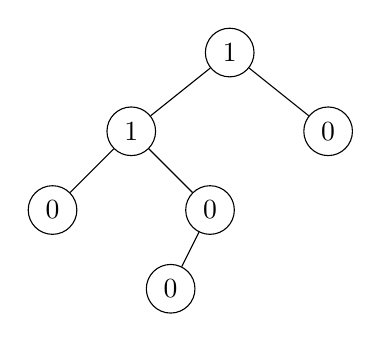
\begin{tikzpicture}[level distance=1cm,
  level 1/.style={sibling distance=2.5cm},
  level 2/.style={sibling distance=2cm},
  level 3/.style={sibling distance=1cm},
every node/.style = {shape=circle, draw, align=center}]

\node{1}
child {
	node {1}
	child {
		node {0}
	}
	child {
		node {0}		
		child {
			node {0}
		}
		child[missing]
	}
}
child {
	node {0}
};
\end{tikzpicture}
\end{figure}

\noindent \textbf{Merk:} En venstreorientert heap forsøker å være ute av balanse (for å gjøre fletting enklere).

\paragraph{Operasjoner}~\\
Hovedoperasjonen på venstreorienterte heaper er \textbf{fletting} (engelsk: merging). Vi kan implementere fletting rekursivt: Når vi skal flette to heaper $ H_1 $ og $ H_2 $ sammenligner vi først røttene. La $ H_1 $ være heapen med minst rot. La så den høyre subheapen til $ H_1 $ være heapen som fremstår ved å flette høyre subheap i $ H_1 $ med hele $ H_2 $. Vi fortsetter slik til problemet er trivielt. Gjennomgående kan vi bytte om høyre og venstre subheap for å bevare strukturkravet (def. pt. 1).

For å \textbf{sette inn} en node i en venstreorientert heap kan vi flette en heap bestående av den ene noden vi vil sette inn, med hele heapen vi vil sette noden inn i.

For å \textbf{fjerne} minste node kan vi ta vekk rota (som vi vet er minst fra def. pt. 2), og flette venstre og høyre subheap.





\subsection{Hashmap (hashtabell)} \label{hashmap}
Sett at vi har en liste med $ n $ elementer. Vi skal søke etter et element $ x $. Hvis vi har implementer lista vår som en array eller lenket liste vil dette ta $ O(n) $ tid. Det vil også operasjoner som sletting, og å sette inn på første ledige plass. Vi ønsker å finne en datastruktur som er bedre på disse tingene. 

Den grunnleggende idéen bak hashtabeller er å la verdien til elementet vi skal sette inn bestemme indexen. Vi bruker en hashfunksjon $ f:\mathbb{N}\rightarrow\mathbb{N} $ på elementet vårt $ x $, og lar $ f(x) $ betegne indexen til elementet i en array. 

\begin{itemize}
\item Når vi oppretter en hashtabell lager vi en ny array som er $ tableSize $ lang. Størrelsen på arrayen er et primtall. 
\item Når vi skal sette inn et element $ x $ i en hashtabell regner vi ut $ f(x) $ og setter $ x $ inn i arrayen på plass $ f(x) $
\item Når vi skal søke etter et element $ x $ i hashtabellen regner vi ut $ f(x) $ og slår opp på den plassen i arrayen. Hvis elementet er der har vi funnet det. Hvis elementet ikke er der må vi muligens sjekke noen andre steder. Hvor vi må lete videre avhenger av hvordan vi håndterer like hashresultater. 
\item Når vi skal fjerne et element $ x $ i en hashtabell søker vi opp elementet i tabellen, og sletter det. 
\end{itemize}

\noindent Et eksempel på en hashfunksjon kan være $ f(x) = x \mod tableSize $

~\\
\subsubsection{Håndtering av like hashresultater}
Hashfunksjoner trenger ikke å være injektive. Det vil si at vi fort kan få $ f(x) = f(y) $ selv om $ x \neq y $. Hvis vi skal sette inn $ y $ i en hashtabell, men plassen med index $ f(y) $ allerede er okkupert av $ x $ må vi finne en ny plass til $ y $. Det kan gjøres på flere måter, vi deler opp i to hovedgrupper: Seperate chaining og probing. 


\paragraph{Seperate chaining}~\\
En mulig løsning på problemet med like hashresultater er å la arrayen vår være en array av lenkede lister. Vi kan dermed ha flere elementer i hver index. Når vi skal sette inn $ x $, regner vi ut $ f(x) $, og setter y bakerst i lista på den plassen. Dermed har det ingenting å si om det eksisterer elementer på indexen eller ikke. 

Problemet med seperate chaining er at vi må tråkke oss gjennom en lenket liste etter at vi har funnet hashresultatet. Dette tar lineær tid (men dog med (forhåpentligvis) færre elementer enn $ n $)


\paragraph{Lineær probing}~\\
En annen mulig løsning på problemet er å gå til plassen bak $ f(x) $, og hvis den er opptatt går vi til indexen bak det igjen. Skulle vi komme til enden av arrayen begynner vi fra toppen igjen. Generelt for probing har vi at plassen vi setter elementet inn på er gitt ved
\[ index = (f(x) + g(k)) \mod{tableSize} \]
der $ f $ er hashfunksjonen, $ g $ er i dette tilfellet $ g(k) = k $, $ k $ er antall skritt vi har tatt fra den opprinnelige indexen (antall ganger vi har støtt på et element) og $ tableSize $ er antall plasser i tabellen. Igjen får vi det problemet at vi i praksis må søke igjennom en liste etter å ha funnet hashresultatet. 

\paragraph{Kvadratisk probing}~\\
Kvadratisk probing ligner veldig på lineær probing, med den forskjellen at $ g(k) = k^2 $. Vi går altså til den plassen som ligger $ 1, 4, 9, ... $ plasser bak $ f(x) $

\paragraph{Dobbel hashing}~\\
Med dobbel hashing har vi en ekstra hashfunksjon $ f_2(x) $ som vi regner ut hvis vi skulle støte på problemer. Vi får da at $ g(k) = k f_2(x) $. Et eksempel på en funksjon $ f_2 $ kan være $ f_2(x) = R-(x \mod R) $ der $ R $ er det største primtallet som er mindre enn $ tableSize $. 

~\\
\subsubsection{Rehashing}
Hvis hashtabellen begynner å bli full kan det lønne seg å rehashe. Det betyr ganske greit å lage en ny tabell med større $ tableSize $ og flytte alle elementet over. Når vi rehasher lager vi som regel en tabell som er ca dobbelt så stor (men fortsatt primtall). Siden $ f $ ofte avhenger av $ tableSize $ må vi regne ut alle hashverdiene på nytt. Rehashing er derfor en ganske dyr affære, så vi gjør det veldig sjeldent, men hvis tabellen begynner å bli for full kan vi tjene ganske mye tid i lengden. 

~\\
\subsubsection{Gode hashfunksjoner}
Vi står helt fritt til å velge hashfunksjoner selv. Gode hashfunksjoner er raske å regne ut, kan gi alle mulige verdier fra $ 0 $ til $ tableSize - 1 $, og har en god fordeling (spredning). utover tabellindexene. 

Ofte bruker vi strenger som nøkler. Vi må derfor ha en måte å regne ut et tall av en tekststreng på. Det kan gjøres på mange måter, her er et par eksempler:
\begin{itemize}
\item Summer verdiene til hvert tegn:
\[ f(x) = \left( \sum_{i=0}^{keyLength-1} = \text{charVal}(key_i) \right) \mod{tableSize} \]
der $ \text{charVal} $ er en funksjon som tilordner en numerisk verdi til hver bokstav, feks ascii/unicode-verdien til tegnet. $ key_i $ betegner det $ i $-te tegnet i $ key $. Denne funksjonen er rask og enkel å implementere, men vil gi dårlig spredning for store tabeller. 
\item En vektet sum av de tre første tegnene:
\[ f(x) = \left( c_1\,\text{charVal}(key_1) + c_2\,\text{charVal}(key_2) + c_3\,\text{charVal}(key_3)\right)  \mod{tableSize} \]
der $ c $-ene er konstanter vi velger. Denne er rask å enkel å beregne, og gir en grei fordeling for tilfeldige strenger, problemet er at naturlig språk ikke er tilfeldig.
\end{itemize}


\subsubsection{Tidsanalyse}
Det er åpenbart at best case tid for innsetting, søking og fjerning i hashtabeller er $ O(1) $. Det oppstår når vi kommer rett til elementet/tom index på første forsøk. Worst case er når vi får kollisjoner på hvert eneste treff, og vi i praksis har en liste. Da vil alle operasjoner på tabellen være $ O(n) $. 

Vi ser at en tabell starter som $ O(1) $, og beveger seg mot $ O(n) $ når den blir fullere. Det er derfor vi ofte velger å rehashe når tabellen blir for full. Selv om rehashing har $ O(n) $ tid, er det en operasjon vi gjør én gang. Det vil forbedre kjøretiden på alle andre operasjoner drastisk, siden det er mindre sannsynlighet for å få kollisjoner i en tabell med mindre tetthet. Som regel prøver vi å holde andelen av tabellen som er opptatt (kalt \say{load factor}, ofte forkortet $ LF $) under en gitt grense. Java sin innebygde \verb|HashMap<K,V>| tvinger $ LF < 0.75 $.





\subsection{Kø/stack} \label{ko_stack}
Kø og stack er to forskjellige typer lister. Felles for dem er at vi kun opererer med én \verb|insert()|- og én \verb|remove()|-metode. Forskjellen er hvilket element vi vil hente ut når vi kaller \verb|remove()|-metoden. Innsetting og fjerning i både kø og stack tar $ O(1) $ tid, siden vi på forhånd vet hvor elementet skal fjernes fra/legges til. 


\subsubsection{Kø (FIFO)}
En kø er en liste der første element inn er det første som kommer ut, derav navnet. Vi kaller også slike lister for FIFO-lister (First In, First Out). Elementene som settes inn stilles bakerst i køen, og når vi henter ut et element starter vi foran. 


\subsubsection{Stack (LIFO)}
En stack (norsk: stabel) er en liste der siste element som settes inn er det første som kommer ut. Slike lister kalles også LIFO-lister (Last In, First Out). Elementene som settes inn legges på toppen av stabelen, og når vi skal hente ut et element henter vi det øverste elementet. 

Konvensjonelt kalles insert-metoden i en stack \verb|push()|, og remove-funksjonen \verb|pop()|

